\documentclass[xcolor=table]{beamer}

\usetheme[secheader,compress]{Madrid} %Primary theme

\usepackage{verbatim}
\usepackage{graphicx}
\usepackage{hyperref}

%% UTM Colors
\definecolor{UTMblue}{rgb}{0.043137, 0.137254, 0.254901}
\definecolor{UTMorange}{rgb}{1.0, 0.509803, 0}

\setbeamercolor{palette primary}{bg=UTMblue,fg=white}
\setbeamercolor{palette secondary}{bg=UTMblue,fg=white}
\setbeamercolor{palette tertiary}{bg=UTMblue,fg=white}
\setbeamercolor{palette quaternary}{bg=UTMblue,fg=white}
\setbeamercolor{structure}{fg=UTMblue} % itemize, enumerate, etc
\setbeamercolor{section in toc}{fg=UTMblue} % TOC sections
\setbeamercolor{title}{fg=UTMorange}

\setbeamercolor{subsection in head/foot}{bg=UTMorange,fg=white}

%%%%%%%%%%% BEGIN MACROS %%%%%%%%%%%%%%%%%%
% frameT: Frame with title
\newcommand{\frameT}[2]{\frame{\frametitle{#1} #2}}

% frameF: Fragile frame with title
\newcommand{\frameF}[2]{
  \begin{frame}[fragile]
    \frametitle{#1}
    #2
  \end{frame}
}

% frameTop: Frame aligned t the top
\newcommand{\frameTop}[2]{\frame[t]{\frametitle{#1} #2}}


\newcommand{\tab}{\hspace{1cm}}

\newcommand{\spaceor}{\hspace{5pt} \textbf{or} \hspace{5pt}}

%%%%%%%%%%% END MACROS %%%%%%%%%%%%%%%%%%%%



\begin{document}

\title{Gardener's Best Friend}

\author{Shakira Perry, Lucy Gauldin, Vrushank Mali, and Chase Duclos}
\institute{UT-Martin}
\date{\today}

%%%%%%%%%%% BEGIN TITLE %%%%%%%%%%%%%%%%%%
\frame{\titlepage}

 %\section{Outline}
%%%%%%%%%%%% END TITLE  %%%%%%%%%%%%%%%%%%


\section{Introduction}
\frameT{Motivation} {
  So why did we pick this project?
\begin{columns}
\column{0.5\textwidth}
   \begin{enumerate}
    \item Love of plants
      \bigskip
    \item Keep plants ALIVE!!!
    \bigskip
    \item Improve plant health
  \end{enumerate}
\column{0.5\textwidth}
    \begin{figure}[H]
    
\includegraphics[width = .7\linewidth]{app_logo.png}
    \end{figure}
    \end{columns}

  
}



\frameT{Project Goals} {
  So what do we think we need to have?
\bigskip

\begin{itemize}
    \item \textbf{Plant Journal}
          \begin{itemize} 
            \item Keep record of plant's health with journal entries.
          \end{itemize}
    \item \textbf{Photo records}
        \begin{itemize}
            \item Journal entries will contain photos that can be updated by the user.
        \end{itemize}

    \item \textbf{Calendar Reminders}
        \begin{itemize}
            \item Depending on the schedule assigned by the user, a reminder will be sent to water their plants.
        \end{itemize}

        \item \textbf{Plant Information}
        \begin{itemize}
            \item If the plant is within the app's database, the user will be presented further information about their plant's care.
        \end{itemize}
        
    
\end{itemize}
}

\begin{frame}[fragile]
\frametitle{Technology}
\begin{columns}
\column{0.5\textwidth}
Technology used:
   \begin{enumerate}
    \item Android Studio
    \item Kotlin programming language
    \item Plant API from Perenual
    \item GitHub
  \end{enumerate}
\column{0.5\textwidth}
    \begin{figure}[H]
    
\includegraphics[width = .8\linewidth]{technologies.png}
    \end{figure}
    \end{columns}
\end{frame}


\frameT{Journey to the App}
{
First Mockup \\

\begin{center}
   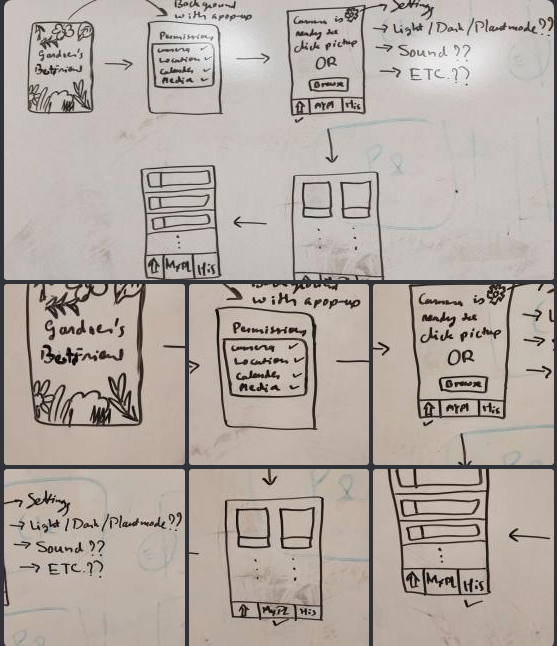
\includegraphics[scale=0.35]{Screenshot 2023-09-30 183429.png}
\end{center}
}

 \frameT{First Splash Screen}
 {
 \begin{center}
   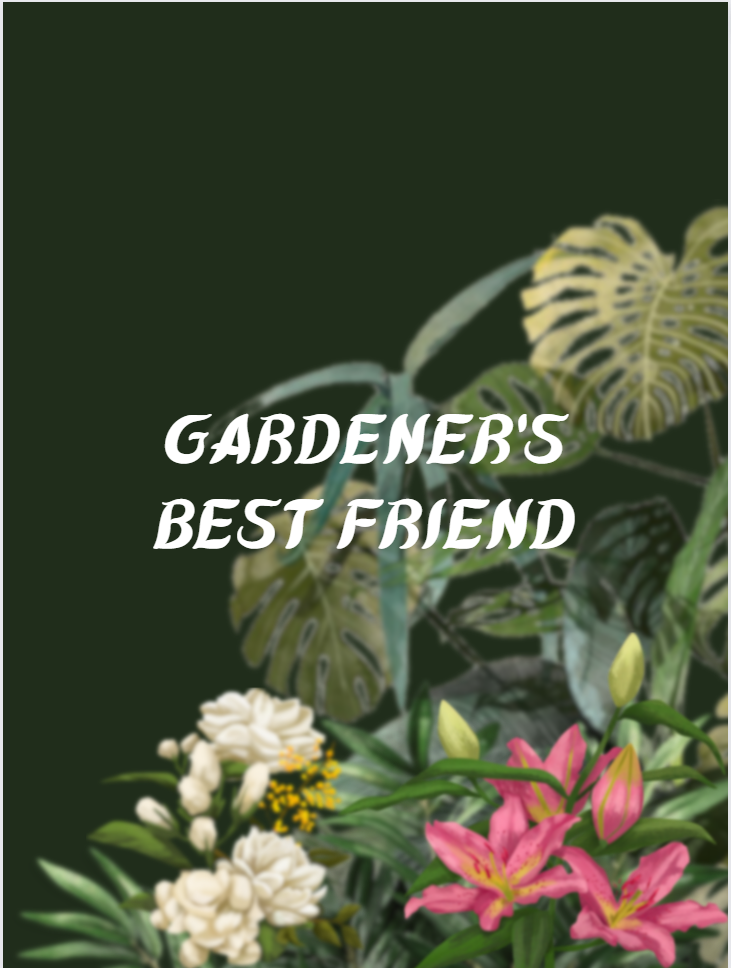
\includegraphics[scale=0.25]{Screenshot 2023-09-30 183202.png}  
 \end{center}    
}

\frameT{First Plant Entry}
{
\begin{center}
    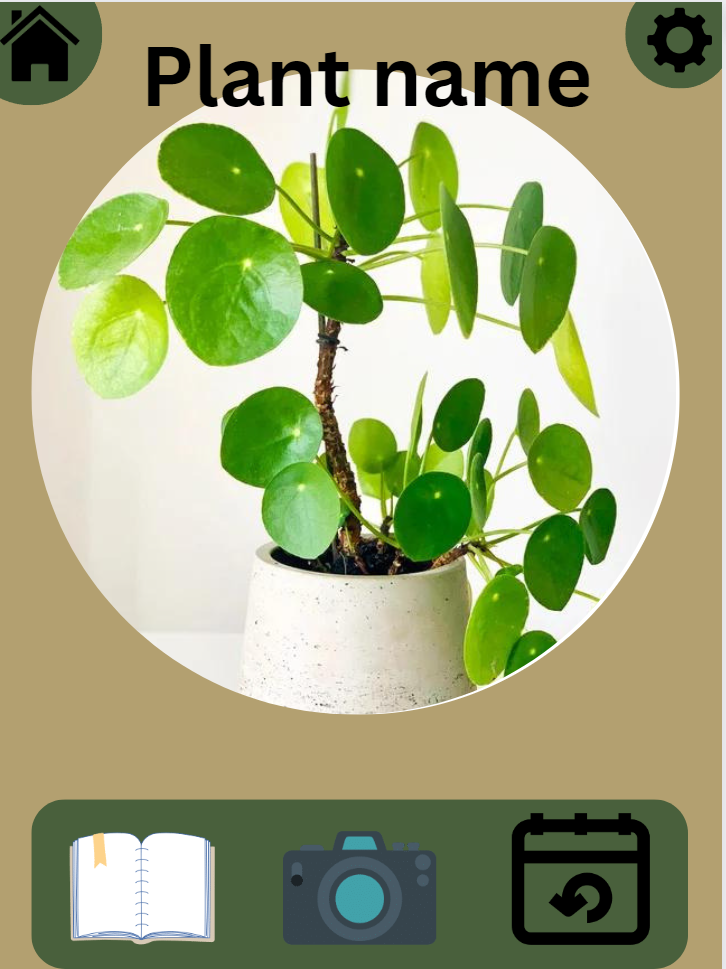
\includegraphics[scale=0.25]{Screenshot 2023-09-30 183239.png}
\end{center}
}


\frameT{Demonstration} {
\begin{center}
  \href{https://www.youtube.com/shorts/_OxIkZ9Jxa0}{Demonstration Video}  
\end{center}

}





\frameT{Results} {
  Describe any results of your work here.

  \bigskip

  Things that worked?

  \bigskip

  Things that didn't work?

  \bigskip
  Challenges? \\
  Getting Android Studio to link with Github for version control \\
  Deciding on what features the app needed
}

\frameT{Conclusions} {
  While it has been a fun project, there is a lot more left to do.
  \begin{itemize}
      \item Send user reminders.
      \item Enable camera/gallery access to input photos into journal entry.
      \item Journal entry storage for retrieval.
      \item Access database with help of API.
  \end{itemize}
}

\frameT{Any Questions?} {
  
  \begin{center}
    Questions?
  \end{center}
  \begin{center}
    Comments?
  \end{center}

  \bigskip
\begin{center}
  Further project/author information: \\
 Wesley Duclos: wescducl@ut.utm.edu \\ Lucy Gauldin: bildgaul@ut.utm.edu \\ Vrushank Mali: vrujmali@ut.utm.edu \\ 
       Shakira Perry: shaaperr@ut.utm.edu

  
    \includegraphics[width=4cm]{happyplant.png}
  \end{center}
}

%\frameF{fragile test} {
%}

%% \frameF{Prolog Family Tree} {
%% \begin{verbatim}
%% hello
%% \end{verbatim}



%% }

%Empty Page
%\frameT{Frame 1}{
%}  


\end{document}